\section{Introducción}

Las \textbf{redes neuronales} son modelos computacionales inspirados originalmente en los mecanismos de aprendizaje y procesamiento de información del cerebro humano \cite{Mculloch43}. Estos modelos, organizados en capas, están formados por un conjunto de unidades de procesamiento simples, comúnmente denominadas neuronas artificiales, que están altamente interconectadas y, mediante un proceso de aprendizaje, son capaces de resolver tareas específicas \cite{patternrecog, pml1Book, Mostafa2012}. Las redes neuronales constituyen uno de los pilares fundamentales del éxito actual del aprendizaje profundo\footnote{El aprendizaje profundo permite que estos modelos computacionales adquieran representaciones jerárquicas con múltiples niveles de abstracción a partir de los datos de entrada \cite{lecun2015deep, SCHMIDHUBER201585}.} y, por extensión, es una de las bases del desarrollo de la inteligencia artificial (IA) \cite{bishop2023learning, prince2023understanding, 2016modernapp}.

\begin{figure}[H]
    \centering
    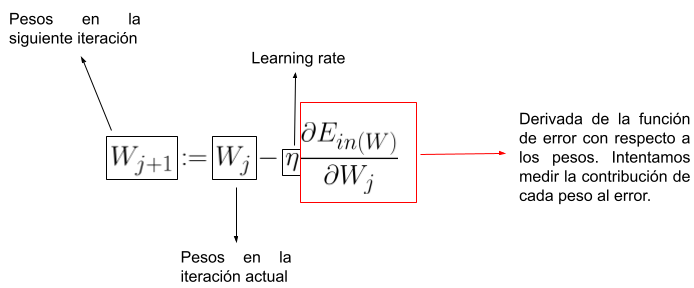
\includegraphics[width=0.9\linewidth]{Plantilla_TFG_latex//imagenes//Inf//Int/gd_bp.png}
    \caption[Aclaración de la diferencia entre el algoritmo de gradiente descendente y \textit{backpropagation}]{En la figura observamos la fórmula de actualización de los pesos de un modelo a través del algoritmo de gradiente descendente. Los elementos se indican en un recuadro señalado con su correspondiente explicación. El elemento señalado en rojo es el correspondiente al algoritmo de \textit{backpropagation}, es decir, usamos este algoritmo para computar esta derivada parcial. Con esta figura se pretende resaltar la diferencia entre el algoritmo de gradiente descendente, utilizado para la optimización de los parámetros en el entrenamiento de modelos, y el algoritmo de \textit{backpropagation}, cuyo fin es el cálculo eficiente del gradiente de una función.}
    \label{fig:gd_bp}
\end{figure}

El \textbf{entrenamiento} de una red neuronal es el proceso por el que optimizamos sus parámetros internos para minimizar una \textbf{función de pérdida} que cuantifica el error entre las predicciones realizadas por la red y las etiquetas reales del conjunto de datos. Este proceso es conceptualizado como un \textbf{problema de optimización} \cite{lecun2015deep}, en el que utilizando un \textbf{algoritmo de aprendizaje} actualizamos iterativamente los parámetros de la red en dirección al mínimo de la función de pérdida. El entrenamiento no sólo busca aprender los patrones en los datos para minimizar el error, sino también garantizar la \textbf{capacidad de generalización} del modelo a nuevos datos \cite{bishop2023learning, GoodFellowBook}.



El algoritmo de aprendizaje más habitual para redes neuronales es el \textbf{gradiente descendente} \cite{ConvexOp, Curry1944GDNoLin} (GD), que calcula iterativamente el gradiente de la función de pérdida con respecto a los parámetros de la red, y los actualiza en dirección opuesta al gradiente para disminuir el error. Existen diferentes versiones del algoritmo según el tamaño del subconjunto de datos usado para calcular el gradiente en cada iteración. Para este cálculo se utiliza el algoritmo de \textit{\textbf{backpropagation}} \cite{rumelbackprop, EffBackProp}, que implica la propagación del error hacia atrás a través de las capas de la red y que implica la aplicación de la regla de la cadena.

\begin{figure}[H]
    \centering
    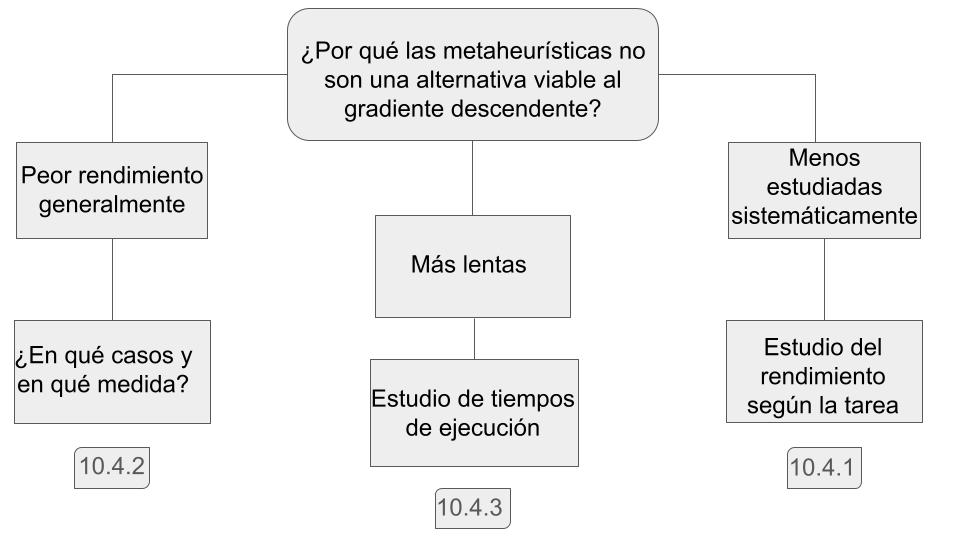
\includegraphics[width=0.9\linewidth]{Plantilla_TFG_latex//imagenes//Inf//Int/fig.jpg}
    \caption[Esquema general de la parte Informática de este TFG con los objetivos parciales a abordar en el mismo]{Esquema general de este TFG con los objetivos parciales a abordar en el mismo. Se parte de la premisa que se plantea en la parte superior a modo de pregunta: ``¿Por qué las metaheurísticas no son una alternativa viable al gradiente descendente [en el momento actual]?". A continuación, planteamos tres posibles respuestas, que son campos de investigación abiertos, y se observan en los tres recuadros centrales. Finalmente, establecemos los enfoques/experimentos desde los que intentaremos abordar la investigación. En la parte baja se indica la sección del TFG en la que se aborda cada punto. No se muestra el objetivo parcial correspondiente a la propuesta algorítmica propia, cuya idea se sintetiza en la Tabla \ref{tab:comp_propias}, se explica en la Sección \ref{sec:propuestas} y se evalúa en la Sección \ref{sec:res_propias}.}
    \label{fig:esquema}
\end{figure}


A pesar de su eficacia y popularidad, el GD presenta varias limitaciones. Una de las principales es su susceptibilidad a \textbf{quedar atrapado en mínimos locales} o puntos de silla \cite{NIPS2014_17e23e50}, especialmente en problema de optimización no convexos, lo que impide alcanzar la solución óptima. Otra es su gran \textbf{sensibilidad}, tanto a los propios hiperparámetros del algoritmo como a los valores iniciales de los parámetros de la red \cite{stabilityProblem2}, que si no se eligen de manera adecuada pueden afectar negativamente al rendimiento e incluso impedir la convergencia. Existen modificaciones del algoritmo que intentan paliar estos problemas al incorporar factores adicionales en la actualización de los pesos.

Por otro lado, las \textbf{metaheurísticas} (MH) \cite{mhhandbook} son técnicas de optimización basadas normalmente en componentes bio-inspirados, que son flexibles y adaptables a gran variedad de problemas. Ofrecen una solución aproximada en un tiempo razonable en muchos problemas cuya solución óptima es computacionalmente inalcanzable, como en problemas NP-Difícil. Son técnicas iterativas que no ofrecen una garantía teórica de hallar una buena solución \cite{MH_desing_imp}, pero a través de restricciones en el algoritmo se espera que lo hagan. Estas estrategias \textbf{no necesitan el uso de gradiente} por lo que exploran el espacio de soluciones de manera más global y no tienen algunas de las restricciones anteriormente mencionadas.





En el presente TFG exploraremos las limitaciones de las técnicas MH como alternativa al GD, realizando un estudio comparativo entre ambos enfoques como se observa de manera esquemática en la Figura \ref{fig:esquema}. Tomaremos como referencia el artículo \cite{MHtrainingClase}, donde se analizan las razones por las que las MH aún no igualan el rendimiento del GD, y plantearemos pruebas experimentales diseñadas para identificar las principales limitaciones de estas técnicas. A su vez, estas pruebas permitirán evaluar las virtudes y defectos de las estrategias MH, con el objetivo de ofrecer propuestas para futuras mejoras en su aplicación. Finalmente, \textbf{propondremos dos técnicas nuevas} a través de combinar MH con el descenso del gradiente, cuyas cualidades se resumen en la Tabla \ref{tab:comp_propias}.







\begin{table}[H]
\centering
\resizebox{\textwidth}{!}{%
\begin{tabular}{|p{3cm}|p{4cm}|p{4cm}|p{4cm}|}
    \hline
    \textbf{Aspecto} & \textbf{Técnicas Clásicas} & \textbf{Metaheurísticas} & \textbf{Propuestas Propias} \\ \hline
    
    \textbf{Fundamento teórico} &
    Basadas en el gradiente. &
    Se basan en heurísticas de búsqueda (aleatorias, evolutivas, inspiradas en la naturaleza, etc.). &
    Combinar el uso del gradiente con mecanismos evolutivos. \\ \hline
    
    \textbf{Ventajas} &
    - Alta eficiencia cuando se dispone de funciones diferenciables. \par
    - Buena capacidad de explotación en zonas prometedoras. \par
    - Mayor conocimiento teórico: comportamiento más predecible, criterios de convergencia más claros y más estudiados.&
    - Permiten explorar grandes espacios de búsqueda sin requerir información del gradiente. \par
    - Flexibles ante problemas complejos o con múltiples óptimos locales. &
    - Toman la fuerza de explotación del gradiente y la capacidad exploradora de las metaheurísticas. \par
    - Flexibles y adaptables. \\ \hline
    
    \textbf{Limitaciones} &
    - Pueden estancarse en óptimos locales si la función es compleja. \par
    - Requieren derivadas (no siempre disponibles o fiables). &
    - Suelen requerir más evaluaciones de la función objetivo. \par
    - No aprovechan información de derivadas incluso si está disponible, lo que puede resultar menos eficiente. &
    Aumenta la complejidad de implementación. \\ \hline
    
    \textbf{Capacidad} &
    Principalmente explotadora: refinan soluciones en regiones vecinas. &
    Principalmente exploradora: buscan soluciones en todo el espacio, reduciendo la probabilidad de caer en óptimos locales. &
    Combina explotación (guiada por el gradiente) con exploración (a través de SHADE, basado en \textit{Differential Evolution}). \\ \hline
    
    \textbf{Algoritmos} &
    Adam \cite{Adam}, NAG \cite{Nesterov}, RMSProp \cite{rmsprop}, AdamW \cite{AdamW} &
    SHADE \cite{shade}, SHADE-ILS\footnotemark \cite{shadeils}&
    SHADE-GD, \par SHADE-ILS-GD. \\ \hline
    

\end{tabular}%
}
\caption[Tabla comparativa entre las técnicas clásicas basadas en gradiente, las metaheurísticas y las dos propuestas algorítmicas propias (SHADE-GD y SHADE-ILS-GD)]{Tabla comparativa entre las técnicas clásicas basadas en gradiente, las metaheurísticas y las dos propuestas algorítmicas propias (SHADE-GD y SHADE-ILS-GD) para el entrenamiento de modelos. Las propuestas híbridas buscan combinar la eficiencia y capacidad explotadora de los optimizadores basados en gradiente con la capacidad exploradora de las metaheurísticas. Este enfoque permite superar algunas limitaciones del gradiente, como el estancamiento en óptimos locales. El análisis detallado de estas propuestas y los resultados empíricos pueden encontrarse en la Sección \ref{sec:propuestas} y la Sección \ref{sec:res_propias}, respectivamente.}
\label{tab:comp_propias}
\end{table}

\footnotetext{Dentro de los algoritmos MH, SHADE-ILS pertenece al grupo de algoritmos meméticos, que sí incorporan búsqueda local, y en particular este algoritmo utiliza información de gradiente.}

\begin{comment}
\begin{figure}[!tbp]
    \centering
    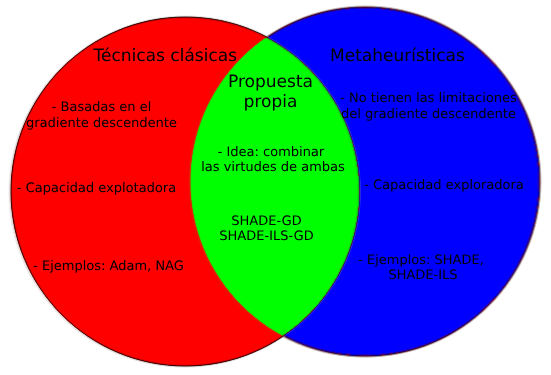
\includegraphics[width=0.9\linewidth]{Plantilla_TFG_latex//imagenes//Inf//Int/propuesta.png}
    \caption[Idea alrededor de las dos propuestas algorítmicas propias]{Diagrama de Venn que muestra de manera esquemática la idea alrededor de las dos propuestas algorítmicas propias (SHADE-GD y SHADE-ILS-GD) para el entrenamiento de modelos. Se pretende combinar la capacidad explotadora y los resultados contrastados de los optimizadores basados en GD junto con la capacidad exploradora y las virtudes de las MH. Estas son, por ejemplo, una capacidad mayor que la del GD a la hora de evadir mínimos locales. El análisis de estas propuestas y los resultados empíricos pueden encontrarse en la Sección \ref{sec:propias} y la Sección \ref{sec:propias}, respectivamente.}
    \label{fig:propuesta}
\end{figure}
\end{comment}


\newpage



\subsection{Motivación}
\label{sec:motinfo}

El ajuste de parámetros es crucial en el aprendizaje profundo ya que determina directamente el rendimiento y la funcionalidad de nuestro modelo. Éste depende de una optimización que permita minimizar en el menor tiempo posible la función de pérdida y capturar los patrones subyacentes a los datos de entrada. Una correcta optimización de los parámetros también mejora la eficiencia computacional e incrementa la fiabilidad de las aplicaciones de aprendizaje profundo.


La optimización de los parámetros de las redes neuronales profundas es inherentemente un problema desafiante. Las superficies de pérdida de estos modelos, sobre todo a medida que aumentan en profundidad (número de capas) y complejidad (número de parámetros), son altamente no lineales y están plagadas de mínimos locales, regiones planas y puntos de silla \cite{NIPS2014_17e23e50}. Además, la alta dimensionalidad del espacio de parámetros, que a menudo llega a millones o miles de millones de dimensiones, incrementa esta dificultad, ya que resulta computacionalmente prohibitivo explorar con técnicas exhaustivas el espacio de búsqueda.

Mientras que las técnicas de optimización basadas en gradientes son eficientes y escalan bien, depender de información local (los gradientes) las hacen vulnerables a ciertas limitaciones como quedar atrapadas en mínimos locales, especialmente en tareas complejas. Por otro lado, las MH son un enfoque completamente distinto, siendo estrategias de búsqueda global que no requieren de información del gradiente, haciéndolas menos sensibles a mínimos locales y potencialmente más robustas navegando superficies de pérdida complejas. 

Aun así estas técnicas son estudiadas de manera menos sistemática que los métodos basados en gradiente, y aunque se conoce que aún no son capaces de igualar el rendimiento de las técnicas clásicas \cite{MHtrainingClase}, son realmente prometedoras y un campo muy activo de investigación, en especial su escalabilidad, coste computacional, y su habilidad de generalización en redes de gran escala \cite{MHtrainingClase}. Además, las diferencias en diseño, requerimientos computacionales, dependencia de hiperparámetros y criterios de comparación o evaluación, hacen difícil comparar objetivamente y de manera no sesgada las causas y contextos específicos de la diferencia de rendimiento entre el GD y las técnicas MH.

Este TFG intentará abordar algunas de estas temáticas abiertas, a través de comparar empíricamente el descenso de gradiente y las técnicas MH en el entrenamiento de redes neuronales profundas. Al hacerlo, se pretende arrojar luz sobre el balance de estos métodos, identificando escenarios donde las MH podrían ofrecer un mejor rendimiento, y proporcionando una comprensión más profunda de las estrategias de optimización en aprendizaje profundo. 





\subsection{Objetivos}\label{sec:objinf}

El objetivo principal de este TFG es evaluar y analizar la eficacia de las técnicas MH para el entrenamiento de redes neuronales profundas. Lo haremos comparándolas con el algoritmo de GD, para tener una mejor comprensión de cuáles son las diferencias principales en el rendimiento de estas dos estrategias y cuáles son las causas de las mismas. De esta manera, se podrían ofrecer modificaciones que mejoren estas técnicas tan prometedoras. Para ello vamos a dividir este objetivo en varios secundarios:

\begin{enumerate}

\item Estudio de la literatura existente, tanto para optimizadores basados en GD clásicos como para el uso de MH en el entrenamiento de modelos de aprendizaje automático.

\item Análisis de los factores que provocan que el rendimiento de las técnicas MH empeore conforme aumenta la complejidad de la tarea, el número de parámetros del modelo y el tamaño del conjunto de datos.

\item Evaluar si existe una diferencia de rendimiento significativa en los modelos entrenados con técnicas MH en función del tipo de tarea a resolver.

\item Medición y análisis de los tiempos de ejecución de las MH, comparando y entendiendo las diferencias con el GD.

\item Propuesta original de dos algoritmos de optimización que hibriden las técnicas MH con el GD.
\end{enumerate}






\subsection{Planificación}

La planificación del TFG ha sido pensada basándonos en los conocimientos previos del grado y en el libro \cite{IngSoft}. Usamos un modelo de cascada retroalimentada, aunque se han realizado varios cambios en la planificación a lo largo del desarrollo. La naturaleza de este proyecto es práctica en el marco de la investigación, por lo que está centrado en la realización y análisis de los experimentos propuestos. Además requiere de una investigación y aprendizaje previos del tema a abordar, seguida de una etapa de diseño de los propios experimentos y el código relacionado.

Una vez implementados y ejecutados los experimentos, analizamos sus resultados y, tras realizar las pertinentes revisiones, podemos decidir modificar ciertos aspectos debido a que se hubieran detectado fallos o identificado potenciales mejoras. Podemos ver una representación gráfica del modelo seguido en la Figura \ref{fig:modcas}.


Las etapas en las que se dividirá el desarrollo son las siguientes:

\begin{enumerate}

\item Investigación: en la primera etapa se buscará bibliografía para profundizar en los conocimientos sobre el entrenamiento de modelos de aprendizaje profundo con GD, se analizará literatura reciente para ver las posibles alternativas y se indagará sobre el estado del arte del entrenamiento de modelos para observar posibles vías de investigación abiertas.

\item Diseño: en base a la información anterior, se concretará el objetivo principal del TFG y en base a él se diseñarán uno o varios experimentos que permitan cumplirlo. En base a esos experimentos, se comenzará a diseñar el código a alto nivel.

\item Implementación: se implementa el código necesario diseñado en la etapa anterior.

\item Ejecución: en esta etapa se ejecutan los experimentos.

\item Análisis: una vez obtenidos los resultados, analizamos los datos para ver si confirmamos las hipótesis de la experimentación, las refutamos, o no obtenemos conclusiones. Durante esta etapa pueden llevarse a cabo, por ejemplo, test estadísticos para confirmar ciertas hipótesis.

\item Revisión: Una vez analizados los datos, vemos la experimentación en su conjunto, analizamos posibles fallos metódicos y en caso de ser necesario modificamos cosas puntuales de las etapas de diseño, implementación y ejecución.

\end{enumerate}

\begin{figure}
    \centering
    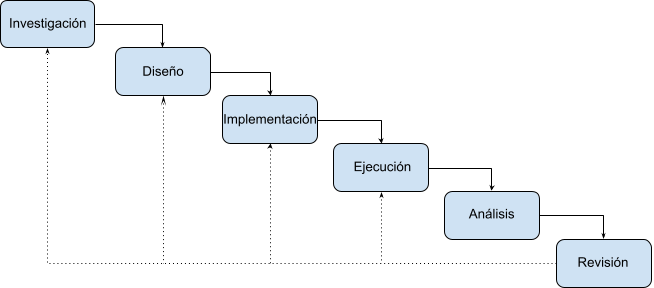
\includegraphics[width=1.06\linewidth]{Plantilla_TFG_latex//imagenes//Inf//Int/workflow.png}
    \caption[Planificación de la parte Informática del presente TFG en modelo de cascada retroalimentada]{Modelo en cascada retroalimentada utilizado en la planificación del proyecto. El proceso inicia con una fase de investigación previa, seguida por el diseño del código y de los experimentos. Luego, se implementa el código necesario para ejecutar los experimentos y, posteriormente, se analizan los resultados obtenidos. En la etapa final de revisión, es posible retroceder a fases anteriores (investigación, diseño, implementación y ejecución) para realizar ajustes y mejoras según sea necesario..}
    \label{fig:modcas}
\end{figure}









El proyecto estaba pensado originalmente para ser empezado en enero y entregarlo en la convocatoria de julio, siguiendo con la planificación que se muestra en la Figura \ref{fig:plan1}. Debido a la carga de trabajo del curso y a que finalmente se comenzó más tarde su trabajo se decidió modificar la propuesta inicial para adaptarla a la realidad, resultando en la planificación que se observa en la Figura \ref{fig:plan2}. En dicha modificación se le asigna más tiempo a la implementación ya que durante los meses de verano disminuyó la cantidad de horas semanal invertidas. A partir de marzo se ha realizado alguna modificación puntual pero no se ha establecido una cantidad de trabajo semanal, por lo que no se computa.

\begin{figure}[!tbp]
    \centering
    \subfloat{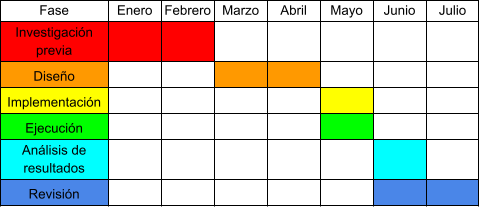
\includegraphics[width=0.75\linewidth]{Plantilla_TFG_latex//imagenes//Inf//Int/plan1.png} \label{fig:plan1}}
    \hfill
    \subfloat{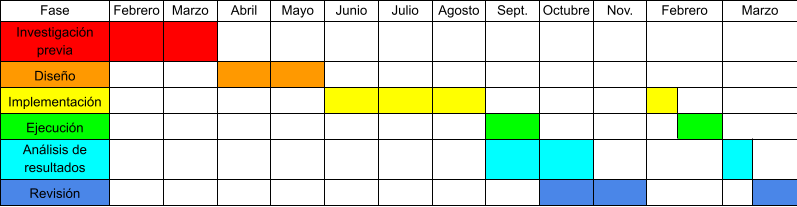
\includegraphics[width=0.9\linewidth]{Plantilla_TFG_latex//imagenes//Inf//Int/plan2.png} \label{fig:plan2}}
    \caption[Diagramas de Gantt de la planificación inicial y final del proyecto]{Diagramas de Gantt de la planificación inicial (arriba) y final (abajo) del proyecto. El primero muestra una planificación inicial más compacta, mientras que el segundo refleja la planificación final ajustada según el progreso y la complejidad de las tareas. Las etapas incluyen: investigación previa, diseño, implementación, ejecución, análisis de resultados y revisión. Los cambios entre ambas versiones evidencian una mayor desagregación de las fases de implementación, ejecución y análisis, lo que permitió una gestión más detallada del tiempo y los recursos. A partir de marzo no se computa ya que, aunque se ha realizado alguna modificación puntual, no se ha establecido una cantidad de trabajo semanal.}
    \label{fig:planesjunto}
\end{figure}

Suponiendo que el sueldo medio de un investigador en España es de unos 30€/h\footnote{\url{https://www.whitecarrot.io/salary-progression/ai-researcher}}, y con una media de 15 horas semanales para el periodo entre febrero y mayo, 5 entre junio y agosto y 30 entre septiembre y marzo (sin contar con diciembre y enero), el coste del personal del proyecto ha resultado ser de 23,400€. Si atendemos a la planificación original, donde se tenía pensado dedicar 20 horas semanales hasta mayo y 15 en junio y julio, el coste del personal hubiera sido de 15,600€, con lo que tendríamos un sobrecoste de 7,800€. 

Para la ejecución de los experimentos se requiere una plataforma que proporcione acceso a hardware en la nube bajo demanda. En este caso se ha seleccionado Paperspace\footnote{\url{https://www.paperspace.com/}} plataforma utilizada en este TFG, aunque en una versión inferior. La elección de una versión superior responde a la necesidad de mayor versatilidad y al supuesto de contar con un presupuesto más amplio. Se ha optado por un plan de suscripción de 34 dólares mensuales (aproximadamente 31.50€). Dado el cronograma del proyecto y considerando que las etapas de investigación y diseño no requieren el uso de la plataforma se ha estimado un periodo de suscripción de 8 meses con un coste total de 252€. En comparación con la planificación inicial que contemplaba únicamente 3 meses de suscripción (94.50€), esto representa un incremento de 157.50€. En consecuencia el presupuesto total estimado para el proyecto asciende a 23,652€.

